\documentclass{book}

\usepackage[spanish]{babel}


\usepackage[letterpaper,top=2cm,bottom=2cm,left=3cm,right=3cm,marginparwidth=1.75cm]{geometry}

\usepackage{amsmath}
\usepackage{graphicx}
\usepackage[colorlinks=true, allcolors=blue]{hyperref}

\title{Accidentes de Tráfico en Nueva Zelanda}
\author{Paola Espinoza Hernández, Jeikel Navarro y Gabriel Sanabria Alvarado}

\begin{document}
\maketitle


\chapter*{Bitácora 1}

\section{Planificación}

\subsection{Pregunta de investigación}
¿Cuáles variables tienen mayor impacto en la severidad de los accidentes de tráfico en Nueva Zelanda?

\subsubsection{Definición de la idea}

La idea principal para esta pregunta de investigación se centra en la identificación y análisis de los factores que influyen en la gravedad de los accidentes de tráfico en Nueva Zelanda. 

\subsubsection{Conceptualización de la idea}

La severidad de los accidentes de tráfico se refiere al grado de daño o consecuencias que resultan de un siniestro vial, pudiendo clasificarse en leves, graves o fatales. Diversos factores pueden influir en esta severidad, incluyendo elementos ambientales, vehiculares, humanos y de infraestructura.

Si bien esta investigación se centra en identificar las variables con mayor impacto en la severidad de los accidentes de tráfico en Nueva Zelanda, el enfoque puede extenderse para incluir análisis comparativos con otros países, evaluar la efectividad de políticas de seguridad vial o desarrollar modelos predictivos de riesgo. Esto permite abordar distintos métodos y perspectivas dentro del tema, volviendo el estudio mucho más profundo para futuras investigaciones.

Este estudio busca proporcionar cierta evidencia empírica para una correcta elaboración de las estrategias de seguridad vial en Nueva Zelanda. Al identificar los factores que impactan principalmente en la severidad de los accidentes, se pueden diseñar políticas públicas más efectivas y medidas preventivas que reduzcan la mortalidad y el impacto socioeconómico de estos incidentes.

\subsubsection{Identificación de tensiones}

En el contexto de esta investigación se pueden identificar diversas tensiones que afectan la severidad de los accidentes. Estas tensiones surgen de la interacción compleja de diferentes variables, lo que complica la predicción y análisis de los accidentes. Un ejemplo a considerar son las condiciones meteorológicas adversas, como lo son la lluvia o la niebla, pueden disminuir la visibilidad y así provocando un aumento a la probabilidad de accidentes graves, pero esto se ve intensificado por la falta de señales de tráfico adecuadas o un control de tráfico deficiente, lo que genera que ocurran accidentes más severos. A su vez, las zonas con límites de velocidad más altos o una velocidad recomendada no respetada en ciertas áreas, como zonas cercanas a peatones o zonas con pendientes pronunciadas, también contribuyen a un aumento en la severidad de los accidentes.

Las condiciones de las calles como superficies mojadas, resbaladizas o mal mantenidas pueden influir significativamente en la severidad del accidente, aumentando la cantidad de lesiones graves o incluso de muertes, además si la velocidad no está dentro de los límites permitidos. Por otro lado, los días festivos pueden llegar a ser un problema a considerar bajo este contexto, esto pues suelen incrementar el tráfico en las carreteras, lo que aumenta el riesgo de fuertes accidentes. También, la presencia de peatones en las zonas de tráfico aumenta el riesgo de accidentes graves, ya que, incluso a velocidades moderadas, el impacto con un peatón puede ser fatal. Este conflicto se intensifica si las zonas peatonales no están bien señalizadas o si los conductores no prestan suficiente atención.

Un punto importante a considerar es el caso de las vías que se encuentran en zonas montañosas, donde las pendientes y la mala calidad del asfalto pueden hacer que los vehículos pierdan el control, y como consecuencia, generando accidentes graves. Las condiciones climáticas como la lluvia pueden agravar este riesgo, lo que genera una mayor severidad en los accidentes en estas zonas. Por último, los accidentes en áreas rurales suelen ser más graves no por la naturaleza del accidente en sí, sino por la falta de accesibilidad rápida a los servicios de emergencia, lo que puede hacer que la respuesta a un accidente sea más lenta, aumentando las probabilidades de lesiones graves o muertes.

\subsubsection{Reformulación de la idea en modo de pregunta}

\begin{enumerate}
    \item ¿Qué variables tienen la mayor influencia en la severidad de los accidentes de tráfico en Nueva Zelanda?
    \item ¿Cómo afectan factores como el clima, el límite de velocidad y las condiciones de la carretera a la gravedad de los accidentes de tráfico en Nueva Zelanda?
    \item ¿Existen patrones entre la presencia de peatones, el tipo de control de tráfico y la gravedad de los accidentes en Nueva Zelanda?
    \item ¿Por qué es importante identificar las variables que influyen en la severidad de los accidentes de tráfico en Nueva Zelanda?
\end{enumerate}

\subsubsection{Argumentación de la pregunta}

\subsubsection{Pregunta 1: ¿Qué variables tienen la mayor influencia en la severidad de los accidentes de tráfico en Nueva Zelanda?}

\textbf{Contraargumentos}
\begin{itemize}
    \item \textbf{Lógica:} ALgunas de las variables puede que estén interconectadas, haciendo más díficil clasificar el impacto directo de cada una de ellas.
    \item \textbf{Ética:} La recopilación de datos puede estar incompleta o incluso sesgada, llegando a afectar los resultados y su validez.
    \item \textbf{Emocional:} Algunas variables podrían llegar a considerarse para la población en general, disminuyendo el interés en la investigación.
\end{itemize}

\textbf{Argumentos}
\begin{itemize}
    \item \textbf{Lógica:} Utilizando modelos estadísticos y aprendizaje automático, se pueden identificar correlaciones significativas entre las variables y la severidad del accidente.
    \item \textbf{Ética:} Se dará uso de fuentes oficiales y métodos rigurosos para garantizar la veracidad de los datos.
    \item \textbf{Emocional:} Comprender los factores más influyentes permitirá implementar medidas preventivas, reduciendo lesiones y muertes.
\end{itemize}

\textbf{Conclusión:} La identificación de variables clave ayudará a diseñar mejores estrategias de seguridad vial. ¿Cómo se pueden optimizar los recursos para maximizar la reducción de accidentes?

\subsubsection{Pregunta 2: ¿Cómo afectan factores como el clima, el límite de velocidad y las condiciones de la carretera a la gravedad de los accidentes de tráfico en Nueva Zelanda?}

\textbf{Contraargumentos}
\begin{itemize}
    \item \textbf{Lógica:} La relación entre estas variables y la severidad del accidente no siempre es directa, ya que otros factores pueden influir.
    \item \textbf{Ética:} La recopilación de datos sobre condiciones climáticas y su correlación con accidentes puede verse afectada por la falta de registros precisos.
    \item \textbf{Emocional:} Algunas personas pueden minimizar el impacto del clima o del estado de las carreteras en los accidentes, atribuyéndolos exclusivamente a la imprudencia.
\end{itemize}

\textbf{Argumentos}
\begin{itemize}
    \item \textbf{Lógica:} Las condiciones climáticas adversas pueden llegar a aumentar el riesgo de accidentes.
    \item \textbf{Ética:} El uso de datos meteorológicos y registros viales confiables permitirá una evaluación objetiva.
    \item \textbf{Emocional:} Crear conciencia sobre estos factores puede incentivar a la creación de políticas enfocadas en la mejora de la infraestructura vial y alertar a los conductores.
\end{itemize}

\textbf{Conclusión:} Analizar estos factores dar inicio a la implementación de políticas de seguridad más adecuadas. ¿Cómo se pueden mejorar las alertas para conductores en condiciones peligrosas?

\subsubsection{Pregunta 3: ¿Existen patrones entre la presencia de peatones, el tipo de control de tráfico y la gravedad de los accidentes en Nueva Zelanda?}

\textbf{Contraargumentos}
\begin{itemize}
    \item \textbf{Lógica:} La relación entre peatones y accidentes puede depender de factores aleatorios como el comportamiento humano.
    \item \textbf{Ética:} Determinar la responsabilidad en los accidentes que involucran peatones puede ser subjetivo.
    \item \textbf{Emocional:} La percepción de seguridad vial varía entre peatones y conductores puede generar conflictos de intereses.
\end{itemize}

\textbf{Argumentos}
\begin{itemize}
    \item \textbf{Lógica:} Los datos pueden revelar patrones en zonas con alta incidencia de atropellos, permitiendo estrategias de mitigación, esto acompañado de estimaciones generadas mediante argumentos estadísticos.
    \item \textbf{Ética:} La transparencia en el análisis de datos garantizará recomendaciones imparciales.
    \item \textbf{Emocional:} Mejorar la seguridad de peatones puede reducir muertes y fomentar un transporte urbano más seguro.
\end{itemize}

\textbf{Conclusión:} Analizar estos patrones contribuirá a aminorar los choques hacia peatones y mejorar la convivencia vial. ¿Qué medidas pueden tomarse para garantizar la seguridad de peatones en zonas de alto tráfico?

\subsubsection{Pregunta 4: ¿Por qué es importante identificar las variables que influyen en la severidad de los accidentes de tráfico en Nueva Zelanda?}

\textbf{Contraargumentos}
\begin{itemize}
    \item \textbf{Lógica:} Se podría pensar que, en lugar de investigar las variables, se deberían tomar medidas generales de seguridad vial sin tomar en cuenta un análisis tan detallado.
    \item \textbf{Ética:} Algunos pueden cuestionar la priorización de ciertos factores sobre otros en la investigación.
    \item \textbf{Emocional:} Las personas pueden no percibir el impacto de estos estudios hasta que enfrentan una situación de riesgo.
\end{itemize}

\textbf{Argumentos}
\begin{itemize}
    \item \textbf{Lógica:} Conocer las variables más influyentes permitirá diseñar estrategias de prevención más efectivas y basadas en datos.
    \item \textbf{Ética:} Una investigación rigurosa asegurará que las recomendaciones sean imparciales y basadas en evidencia.
    \item \textbf{Emocional:} Una considerable disminución de la severidad de los accidentes impactará positivamente en la calidad de vida de las personas.
\end{itemize}

\textbf{Conclusión:} Identificar estas variables permitirá tomar decisiones informadas para reducir los accidentes. ¿Cómo se pueden comunicar estos hallazgos para generar conciencia y cambios en la sociedad?

\subsubsection{Argumentación a través de datos}

\section{Revisión bibliográfica}

Se buscaron términos relacionados a accidentes viales, como el uso del cinturón, las causas y consecuencias de estos accidentes, y la manera en que estos afectan a los involucrados.

\subsubsection{Estimación de probabilidades de accidentes basada en estados de tráfico en autopistas urbanas}
\textbf{Autor:} Cristian Nicolás Zúñiga González

\textbf{Año:} 2014

\textbf{Tema:} Impacto de los estados de tráfico en la ocurrencia y severidad de accidentes

\textbf{Forma de organizarlo:}

\begin{itemize}
\setlength{\itemindent}{0.5in}
    \item \textbf{Cronológico:} datos del 2012 y primera semana del 2013
    \item \textbf{Metodológico:} Calibración de modelos de elección discreta
    \item \textbf{Temático:} Modelos de elección discreta
    \item \textbf{Teoría:} Modelos para estimar el impacto de diversas variables en la ocurrencia y severidad de accidentes
\end{itemize}

\textbf{Resumen en una oración:} La siniestralidad y severidad de un accidente se ve afectada por el estado del tráfico.

\textbf{Argumento central:} Los estados de transición generan más riesgo de ocurrencia para todos los accidentes.

\textbf{Problemas con el argumento o el tema:} Aunque todos los indicadores mejoran cuando la muestra crece, presentan problemas ante una especificación más desagregada. La vía de estudio, Autopista Central de Santiago en Chile, no posee características desafiantes relacionadas a las condiciones climáticas o la geometría.

\textbf{Resumen en un párrafo:} Entre 2006 y 2012, la siniestralidad en la Autopista Central de Santiago tuvo una  tasa de aumento mayor a la tasa de crecimiento de vehículos, con accidentes recurrentes en lugares o condiciones similares. Se ha detectado anteriormente una relación entre el estado de tráfico y condiciones climáticas y la ocurrencia de accidentes, pero sin discriminar la severidad. Este estudio no solo clasifica los accidentes según su gravedad, sino que también amplía la evaluación del costo social al incluir los efectos de la congestión por bloqueos viales. Se concluye que factores como pendientes descendentes, cambios bruscos de velocidad, alta desviación estándar de velocidad y tramos largos incrementan la probabilidad de accidentes. Además, los estados de tráfico más riesgosos son "cuello de botella", "congestión" y, especialmente, "final de cola", este último asociado a una mayor probabilidad de heridos en pendientes descendentes. Por último, la variabilidad en la velocidad y ajustes frecuentes en ella también elevan el riesgo, evidenciando que la combinación de dinámicas de flujo y diseño vial influye en la siniestralidad.

\subsubsection{Analysis of the factors affecting the severity of two-vehicle crashes}
\textbf{Autor:} Alejandro Ángel, Mark Hickman

\textbf{Año:} 2008

\textbf{Tema:} Factores que afectan la severidad de accidentes vehiculares

\textbf{Forma de organizarlo:}

\begin{itemize}
\setlength{\itemindent}{0.5in}
    \item \textbf{Cronológico:} 2008, con datos de 1995 a 2004
    \item \textbf{Metodológico:} Modelo logit multinomial (para severidad de heridas), regresión lineal (costos)
    \item \textbf{Temático:} Modelación
    \item \textbf{Teoría:} Modelación de impacto en severidad de accidentes
\end{itemize}

\textbf{Resumen en una oración:} El tipo de choque tiene un impacto muy significativo en la severidad del accidente.

\textbf{Argumento central:} Existen muchos factores, tanto de comportamiento personal, características vehículares y de tipo de choque, que afectan la severidad de los accidentes de tráfico.

\textbf{Problemas con el argumento o el tema:} Se considera únicamente el costo de las heridas, no el costo social de la obstrucción vial causada por el choque. El modelo lineal de costos podría ser una hipersimplificación, y no reflejar el verdadero costo.

\textbf{Resumen en un párrafo:} Los accidentes vehículares poseen muchos factores que pueden afectar el resultado de este. Entre estos, destacan el tipo de choque, como el choque de cabeza, que puede incrementar más de 56 veces la fatalidad comparada al choque por la parte trasera del vehículo. Además, el uso de cinturón de seguridad disminuye la severidad del choque, mientras que el estar alcoholizado la aumenta. Adicionalmente, es importante diferenciar las consecuencias para cada participante, pues en los choques de vehículos grandes, estos reducen la severidad para quien los ocupa, pero aumenta la de los demás participantes. 

\subsubsection{Variables predictoras de víctimas graves, críticas o fallecidas en los accidentes de tráfico en Extremadura}
\textbf{Autores:} José Antonio Morales Gabardino, Laura Redondo-Lobato, Francisco Buitrago-Ramírez

\textbf{Año:} 2019

\textbf{Tema:} Variables predictoras de la severidad de accidentes de tráfico

\textbf{Forma de organizarlo:}

\begin{itemize}
\setlength{\itemindent}{0.5in}
    \item \textbf{Cronológico:} datos del 2012 al 1015
    \item \textbf{Metodológico:} Regresión logística binaria
    \item \textbf{Temático:} Predicción de severidad de accidentes vehiculares
    \item \textbf{Teoría:} Factores de riesgo en accidentes viales
\end{itemize}

\textbf{Resumen en una oración:} Los accidentes interurbanos, la edad y la zona aumentan la gravedad y mortalidad vial.

\textbf{Argumento central:} Los accidentes de tránsito interurbanos tienen mayor gravedad y mortalidad que los urbanos, siendo el tipo de accidente, la edad y la ubicación importantes factores predictivos de su severidad.

\textbf{Problemas con el argumento o el tema:} La base de datos utilizada no posee registro del sexo de los accidentados, variabe que parece estar ausente en varios otros estudios. Estos datos tampoco incluyen la evolución final de los pacientes, de modo que no se puede evaluar la repercusión socioeconómica de estos accidentes, y la posible subestimación de fallecidos, pues solo se registran los fallecidos al momento de la atención inicial.

\textbf{Resumen en un párrafo:} En el artículo se analiza si el tipo de accidente (urbano o interurbano), la edad o la atención médica influyen en el resultado del mismo. Se concluye que la mayoría de los accidentes son de tipo interurbano y que estos presentan un mayor porcentaje de gravedad en comparación con los ocurridos en zonas urbanas.El tipo de accidente destaca como una variable predictora relevante, ya que puede incrementar el riesgo de fallecimiento en un $74,5\%$.Asimismo, tanto la edad como las zonas de influencia aumentan la probabilidad de accidentes graves o críticos, por lo que estos factores también deberían considerarse para predecir la severidad de los siniestros viales.

\section{UVE de Gowin}

\begin{figure}
\centering
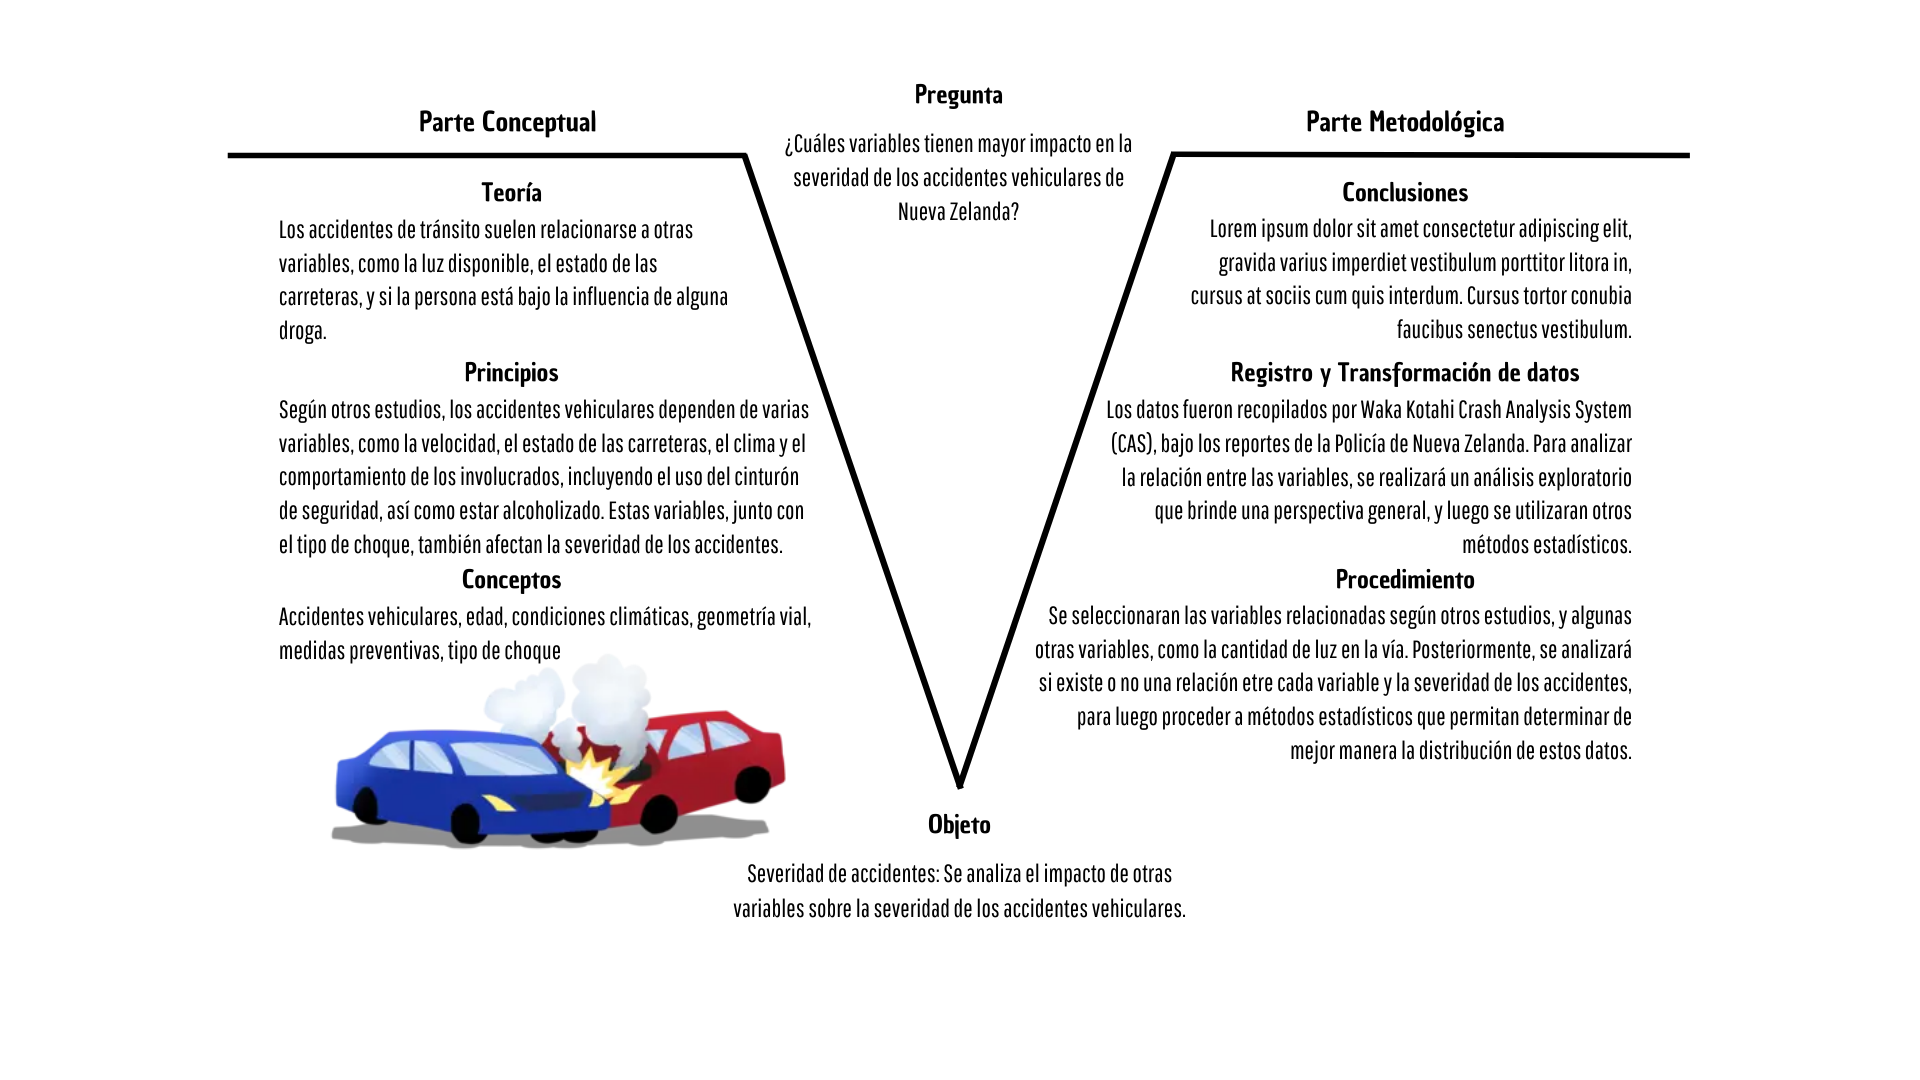
\includegraphics[width=1\linewidth]{V_Gowin_b1.png}
\caption{\label{fig:Gowin}V de Gowin}
\end{figure}

\subsection{Parte de escritura}

Los accidentes de tráfico representan una de las principales causas de muertes y lesiones en todo el mundo. En el caso de Nueva Zelanda, la seguridad vial ha sido una preocupación constante, y se ha buscado implementar diversas estrategias para reducir la siniestralidad en las carreteras. Sin embargo, para mejorar la efectividad de estas estrategias, es fundamental tratar de identificar cuáles son las variables que llegan a tener una mayor influencia o impacto en la severidad de los accidentes. De manera que lo que este trabajo busca es tratar de responder a la pregunta: ¿Cuáles variables tienen mayor impacto en la severidad de los accidentes de tráfico en Nueva Zelanda?

De acuerdo con {BuitragoRamírezFrancisco2019Vpdv}, los diversos factores que podrían llegatr a influir en la severidad de un accidente de tránsito estan los factores humanos, vehiculares, ambientales y de infraestructura. Entres ellos más especificamente se encuentra la atención, concentración y condición psíquico-física del conductor, las características de los vehículos, los objetos y la carga transportada, las condiciones meteorológicas, el ámbito urbano o interurbano en el que ocurre el accidente y el estado de las carreteras.

Así mismo, en busca de garantizar la calidad y veracidad del análisis, este trabajo utilizará como fuente principal los datos provenientes de la Agencia de Transporte Waka Kotahi de Nueva Zelanda. De esta forma, como el objetivo es tratar de determinar qué variables tienen llegan a tener un mayor impacto o incidencia en la severidad de los accidentes de tráfico mediante el uso de métodos estadísticos rigurosos que permitan establecer si existe una relación significativa entre las variables analizadas y la severidad de los accidentes.

Para ello, se plantea desde el inicio las variables de interes que podrían tener un impacto significativo en la severidad de los accidentes, esto al tomar en cuenta que la base de datos cuenta con 72 distintas variables:

\begin{itemize}
    \item Velocidad recomendada
    \item Recuento de victimas fatales
    \item Periodo de vacaciones
    \item Iluminación
    \item Recuento de victimas con lesiones menores
    \item Peaton
    \item Superficie de la carretera
    \item Recuento de victimas con lesiones graves
    \item Límite de velocidad
    \item Clima
\end{itemize}

A su vez, para llevar acabado este propósito de determinar cuáles de estas variables tienen una relación estadísticamente significativa con la severidad del accidente, se emplearán diferentes métodos de análisis de datos, entre ellos:

\begin{itemize}
    \item \textbf{Prueba Chi-cuadrado}: se utiliza para evaluar la independencia entre variables categóricas.
    \item \textbf{Tablas de contingencia}: permiten observar distribuciones conjuntas de variables y detectar patrones de asociación.
    \item \textbf{Prueba t de Student}:  se usa cuando no conocemos ni la media ni la desviación estándar de nuestra población.
    \item \textbf{P-value}: Sirve para determinar la significancia estadística de los resultados obtenidos en los análisis previos, estableciendo si la relación entre variables es lo suficientemente fuerte como para no ser atribuida al azar.
\end{itemize}

Además, el estudio tomará como referencia trabajos previos, como el de {BuitragoRamírezFrancisco2019Vpdv}, que encontró que ciertos factores aumentan significativamente el riesgo de que una víctima resulte fallecida o termine en un estado crítico tras un accidente. Por ejemplo, determinó que los accidentes interurbanos incrementan en un 74.5\% el riesgo de fatalidad en comparación con los urbanos, y que en ciertas zonas de alta incidencia este riesgo puede duplicarse o cuadruplicarse.

Por lo que, identificar las variables que tienen un mayor impacto en la severidad de los accidentes de tráfico permitirá la implementación de estrategias de prevención más efectivas. Esto contribuirá a optimizar la asignación de recursos para la reducción de accidentes, disminuyendo tanto el número de incidentes como la cantidad de personas heridas o fallecidas como consecuencia de los mismos. Además, los hallazgos de este estudio pueden servir como base para futuras investigaciones en seguridad vial y políticas públicas.

\bibliographystyle{plain}
\bibliography{referencias}
\nocite{*}

\end{document}